\documentclass[listings]{labreport}
\usepackage{amsmath}
\subject{Тестирование программного обеспечения}
\titleparts{Лабораторная работа №3}{Вариант 661}
\students{Лабушев Тимофей}

\usepackage{longtable}
\usepackage{enumitem}

\usepackage{array}
\newcolumntype{L}[1]{>{\raggedright\let\newline\\\arraybackslash\hspace{0pt}}m{#1}}

\begin{document}

\maketitlepage

\section*{Задание}

Сформировать варианты использования, разработать на их основе тестовое покрытие и провести функциональное тестирование интерфейса сайта согласно варианту:
\begin{verbatim}
Вариант №661: ADVEGO. Копирайтинг, рерайтинг, переводы. - http://advego.ru/
\end{verbatim}

\begin{enumerate}
\item Тестовое покрытие должно быть сформировано на основании набора прецедентов использования сайта.
\item Тестирование должно осуществляться автоматически - с помощью системы автоматизированного тестирования Selenium.
\item Тесты должны исполняться в браузерах Firefox и Chrome.
\item Предполагается, что тестируемый сайт использует динамическую генерацию элементов на странице, т.е. выбор элемента в DOM должен осуществляться не на основании его ID, а с помощью XPath.
\end{enumerate}

\section*{Диаграмма прецедентов использования сайта}

\begin{center}
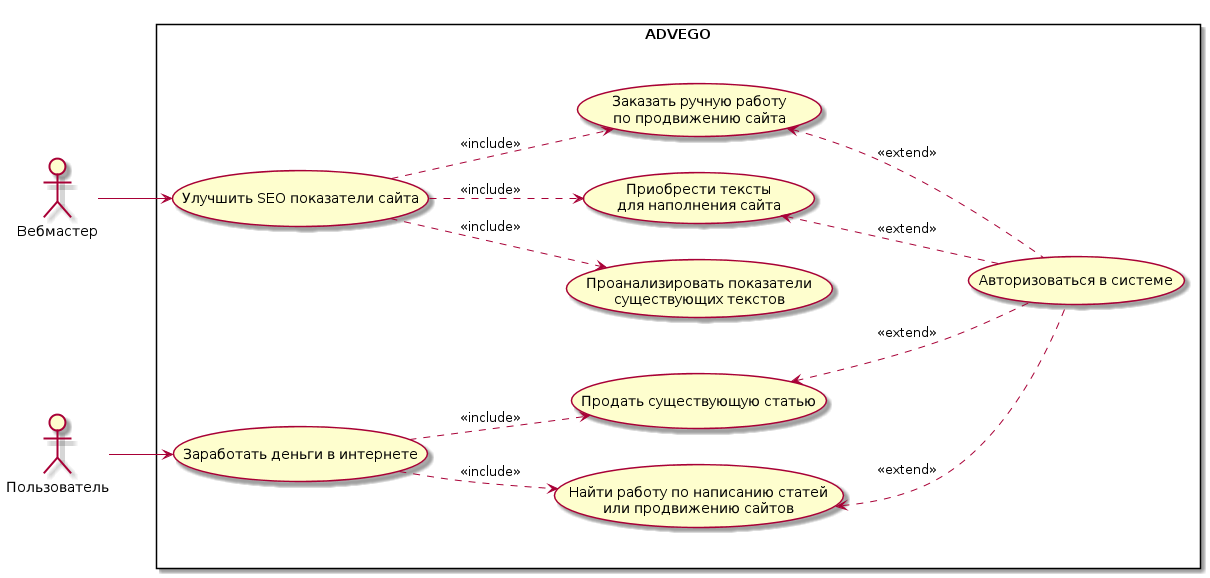
\includegraphics[width=\textwidth]{Lab3.png}\\
Рисунок 1. Диаграмма прецедентов использования тестируемого сайта
\end{center}

\newpage
\section*{Описание тестового покрытия}

Согласно прецедентам использования сайта были разработаны следующие сценарии тестирования:

\renewcommand{\arraystretch}{1.5}
\noindent
\begin{longtable}{L{4.5cm} L{12cm}}
\hline
\textbf{Прецедент \newline (класс сценариев)} & \textbf{Название и описание сценариев тестирования} \\\hline
Проанализировать показатели существующих текстов
  \newline {\small\verb|(SeoAnalysisTest)|} &
\begin{itemize}[noitemsep,topsep=0em,leftmargin=*]
 \item {\small\verb|it spell checks user-provided texts in russian|}\newline
   Анализатор текстов находит опечатки в текстах на русском языке
 \item {\small\verb|it spell checks user-provided texts in english|}\newline
   Анализатор текстов находит опечатки в текстах на английском языке
 \item {\small\verb|it provides character and word statistics|}\newline
   Анализатор текстов составляет базовую статистику (количество символов и слов)
 \item {\small\verb|it analyzes word frequencies ignoring stop words|}\newline
   Анализатор текстов составляет таблицу ключевых слов (исключая стоп-слова)
 \item {\small\verb|it shows an error message when the text is empty|}\newline
   Анализатор показывает осмысленное сообщение об ошибке при запуске без текста
\end{itemize}
  \\\hline
Приобрести тексты для наполнения сайта
  \newline {\small\verb|(MarketplaceTest)|} &
\begin{itemize}[noitemsep,topsep=0em,leftmargin=*]
 \item {\small\verb|it allows users to filter articles by keywords|}\newline
   Пользователь может искать выставленные на продажу статьи по ключевым словам
 \item {\small\verb|it allows users to sort articles by price|}\newline
   Пользователь может сортировать выставленные на продажу статьи по цене
 \item {\small\verb|it allows users to add articles to cart|}\newline
   Пользователь может добавлять статьи в корзину
\end{itemize}
  \\\hline
Заказать ручную работу по продвижению сайта
  \newline {\small\verb|(OrderCreationTest)|} &
\begin{itemize}[noitemsep,topsep=0em,leftmargin=*]
 \item {\small\verb|it shows default order parameters when the page is opened|}\newline
   При открытии страницы заказ уже заполнен шаблонными значениями
 \item {\small\verb|it fills in order parameters based on the selected template|}\newline
   Параметры заказа автоматически изменяются при выборе другого шаблона
 \item {\small\verb|it allows users to search through templates|}\newline
   Пользователь может искать подобрать шаблон заказа, используя поиск
\end{itemize}
  \\\hline
Найти работу по написанию статей или продвижению сайтов
  \newline {\small\verb|(JobSearchTest)|} &
\begin{itemize}[noitemsep,topsep=0em,leftmargin=*]
 \item {\small\verb|it allows users to sort jobs by price|}\newline
   Пользователь может сортировать доступные заявки по оплате за выполнение
 \item {\small\verb|it allows users to filter jobs by category|}\newline
   Пользователь может искать работу в подходящих ему категориях
\end{itemize}
  \\\hline
Продать существующую статью
  \newline {\small\verb|(ListingCreationTest)|} &
\begin{itemize}[noitemsep,topsep=0em,leftmargin=*]
 \item {\small\verb|it allows users to submit new articles to marketplace|}\newline
   Созданная пользователем статья проверяется на соответствие базовым критериям
   (минимальная длина текста, правильно выставленные метаданные) и помещается в магазин
\end{itemize}
  \\\hline
Авторизоваться в системе
  \newline {\small\verb|(SignInTest)|} &
\begin{itemize}[noitemsep,topsep=0em,leftmargin=*]
 \item {\small\verb|it allows users to sign in via the login popup|}\newline
   Пользователь может войти в систему, открыв модальное окно авторизации и введя данные
   своей учетной записи
 \item {\small\verb|it shows an error message when entering invalid credentials|}\newline
   Система показывает осмысленное сообщение об ошибке при вводе неверных данных
   учетной записи
\end{itemize}
  \\\hline
\end{longtable}

\section*{Результаты тестирования}

В ходе тестирования было разработано 18 тестовых сценариев, каждый из которых выполняется
в бразуерах Chrome (с помощью ChromeDriver) и Firefox (с помощью GeckoDriver).

Полностью автоматическое тестирование оказалось нереализуемым из-за применения
на различных страницах сайта системы reCAPTCHA для защиты от ботов.
Полученные сценарии можно считать \textit{автоматизированными}: при запуске каждого из них
открывается новое окно бразуера, и в случае появления запроса ввода капчи тестировщик должен
вручную ответить на него. По прохождении теста окно браузера закрывается.

Помимо этого, тестовое покрытие существенно ограничивается отсутствием доступа к привилегированным
учетным записям. К примеру, новое объявление о работе размещается публично не моментально,
а лишь после прохождения ручной проверки, что подразумевает наличие роли \textit{модератора}.
Однако составить для этой роли прецеденты и разработать автоматизированные тесты не представляется возможным,
так как интерфейс модерации полностью закрыт для стороннего тестировщика.

\section*{Исходный код}

\verb|https://github.com/timlathy/itmo-fourth-year/tree/master/Software-Testing-7th-Term/Lab3|

\section*{Выводы}

В ходе выполнения работы была рассмотрена система автоматизации действий веб-браузера \textit{Selenium}
в контексте написания функциональных тестов интернет-сайтов с пользовательским взаимодействием.

При написании тестов был изучен шаблон \textit{page object}, который позволяет отделить логику тестов
от разметки веб-страницы, что облегчает дальнейшую поддержку тестовых сценариев.

Был также сделан вывод, что стороннее функциональное тестирование веб-приложений малоэффективно.
Отсутствие знаний о системе и трудности получения доступа к ней уменьшают возможное тестовое покрытие.
Подобные условия тестирования подходят скорее для аудитов безопасности системы, в частности, довольно
эффективного метода испытания на проникновение (\textit{penetration testing}).

\end{document}
